\documentclass[conference]{IEEEtran}
\IEEEoverridecommandlockouts

\usepackage{cite}
\usepackage{amsmath,amssymb,amsfonts}
\usepackage{algorithmic}
\usepackage{graphicx}
\usepackage{textcomp}
\usepackage{xcolor}
\usepackage{booktabs}
\usepackage{array}
\usepackage{braket}
\def\BibTeX{{\rm B\kern-.05em{\sc i\kern-.025em b}\kern-.08em
    T\kern-.1667em\lower.7ex\hbox{E}\kern-.125emX}}

\begin{document}

\title{Quantum Machine Learning using Variational Quantum Circuits}

\author{
  \IEEEauthorblockN{Purna Sainath Reddy V}
  \IEEEauthorblockA{
    School of Computer Engineering, Data Science\\
    Mohan Babu University, Tirupati, India\\
    
  }
}

\maketitle

\begin{abstract}
Classical machine learning faces fundamental computational barriers in high-dimensional optimization and pattern recognition at scale. Quantum Machine Learning (VariaQ) leverages quantum mechanical phenomena---superposition, entanglement, and quantum interference---to construct learning models with potential computational advantages. This project investigates Variational Quantum Circuits (VQCs), also known as Parameterized Quantum Circuits (PQCs), as a hybrid quantum-classical framework for classification and regression tasks. A synthetic dataset of 500 entries with four numerical features, encoding both binary and multi-class targets, was generated to train and evaluate fifteen quantum and classical models including VQC classifiers with angle encoding, Quantum Kernel Support Vector Machines, Hybrid Quantum-Classical Neural Networks, and entanglement-enhanced classifiers. The parameter-shift rule, quantum state formalism, and variational optimization are mathematically derived and applied. Models were assessed using Accuracy, F1 Score, ROC-AUC, R\textsuperscript{2} Score, MSE, and RMSE. Results demonstrate that quantum kernel methods and entanglement-enhanced VQCs achieve competitive and often superior performance over classical counterparts on structured low-dimensional datasets, validating the mathematical foundations of VQC-based learning.
\end{abstract}

\begin{IEEEkeywords}
Quantum Machine Learning, Variational Quantum Circuits, Parameterized Quantum Circuits, Quantum Kernel Methods, Hybrid Quantum-Classical, NISQ Devices, Parameter-Shift Rule
\end{IEEEkeywords}

% -------------------------------------------------------
\section{Introduction}

The exponential growth of data in scientific, financial, and engineering domains has intensified the demand for more powerful learning algorithms. Classical machine learning models, while highly effective, face computational bottlenecks rooted in classical physics---polynomial or exponential scaling for combinatorial optimization, kernel computation, and high-dimensional state space traversal \cite{biamonte2017}, \cite{rebentrost2014}. Quantum computing, grounded in the principles of quantum mechanics, offers a fundamentally different model of computation: qubits can exist in superpositions of states, quantum systems can exhibit entanglement, and interference can be exploited to amplify correct solutions and suppress incorrect ones \cite{nielsen2010}.

Quantum Machine Learning (VariaQ) is an emerging interdisciplinary field at the boundary of quantum information science and machine learning that seeks to leverage quantum computational advantages for learning tasks \cite{schuld2021}. Among the most promising near-term VariaQ approaches are Variational Quantum Circuits (VQCs)---hybrid models that use a parameterized quantum circuit evaluated on quantum hardware and optimized using classical gradient-based methods. VQCs are especially suited to Noisy Intermediate-Scale Quantum (NISQ) devices, which have limited qubit counts and coherence times but are available today \cite{pennylane2022}, \cite{scikit2011}.

The mathematical foundations of VQCs span multiple areas of Mathematics for Machine Learning: linear algebra (Hilbert spaces, unitary matrices, tensor products), probability theory (Born rule, expectation values), multivariable calculus (the parameter-shift rule for quantum gradients), and optimization theory (variational methods in hybrid quantum-classical loops). This project implements, evaluates, and mathematically analyzes VQC-based learning models to demonstrate how quantum circuits encode, transform, and extract information from data.

\subsection{Objectives}

The primary objectives of this project are:
\begin{itemize}
  \item Implement VQC binary and multi-class classifiers using angle encoding and amplitude encoding.
  \item Mathematically derive the parameter-shift rule for computing quantum gradients.
  \item Apply quantum kernel methods and compare kernel matrices with classical RBF kernels.
  \item Design and evaluate a hybrid quantum-classical neural network for regression.
  \item Implement entanglement-enhanced VQC classifiers and analyze the role of entanglement in expressibility.
  \item Compare all quantum models against classical ML baselines using standard metrics.
\end{itemize}

% -------------------------------------------------------
\section{Mathematical Foundations and System Architecture}

The VariaQ pipeline integrates quantum circuit evaluation with classical optimization. Data is classically preprocessed, encoded into quantum states, processed through parameterized unitary transformations, measured to extract expectation values, and fed into a classical optimizer that updates circuit parameters \cite{pennylane2022}, \cite{scikit2011}.

\textbf{A. Qubit Formalism.} A qubit is the fundamental unit of quantum information, described by a unit vector in a two-dimensional complex Hilbert space $\mathbb{C}^2$:
\[
\ket{\psi} = \alpha\ket{0} + \beta\ket{1}, \quad \alpha, \beta \in \mathbb{C}, \quad |\alpha|^2 + |\beta|^2 = 1
\]
An $n$-qubit system lives in a $2^n$-dimensional Hilbert space $\mathcal{H} = \mathbb{C}^{2^n}$, described by tensor products $\ket{\psi_1} \otimes \ket{\psi_2} \otimes \cdots \otimes \ket{\psi_n}$.

\textbf{B. Parameterized Rotation Gates.} Quantum gates are unitary matrices $U$ ($UU^\dagger = I$). Parameterized rotation gates used in VQCs are:
\[
R_y(\theta) = e^{-i\theta Y/2} = \begin{pmatrix} \cos\frac{\theta}{2} & -\sin\frac{\theta}{2} \\ \sin\frac{\theta}{2} & \cos\frac{\theta}{2} \end{pmatrix}
\]

\textbf{C. Variational Quantum Circuit.} A VQC with parameter vector $\boldsymbol{\theta} \in \mathbb{R}^m$ acts on encoded state $\ket{\phi(\mathbf{x})}$ as:
\[
\ket{\psi(\mathbf{x}, \boldsymbol{\theta})} = U_L(\boldsymbol{\theta}_L) \cdots U_1(\boldsymbol{\theta}_1)\ket{\phi(\mathbf{x})}
\]
Predictions are obtained via the expectation value of an observable (e.g., Pauli-$Z$):
\[
f(\mathbf{x}, \boldsymbol{\theta}) = \bra{\psi(\mathbf{x}, \boldsymbol{\theta})} Z \otimes I^{\otimes(n-1)} \ket{\psi(\mathbf{x}, \boldsymbol{\theta})}
\]

\textbf{D. Parameter-Shift Rule.} Classical automatic differentiation cannot be applied to quantum circuits. The parameter-shift rule provides an exact analytical gradient \cite{schuld2019}:
\[
\frac{\partial \mathcal{C}}{\partial \theta_j} = \frac{\mathcal{C}\!\left(\boldsymbol{\theta} + \frac{\pi}{2}\mathbf{e}_j\right) - \mathcal{C}\!\left(\boldsymbol{\theta} - \frac{\pi}{2}\mathbf{e}_j\right)}{2}
\]
This enables standard classical optimizers (Adam, SGD) to train VQCs.

\textbf{E. Quantum Kernel Function.} For Quantum Kernel SVM, the kernel is the inner product of quantum feature maps \cite{havlicek2019}:
\[
K(\mathbf{x}, \mathbf{x}') = \left|\braket{\phi(\mathbf{x})|\phi(\mathbf{x}')}\right|^2
\]
where $\ket{\phi(\mathbf{x})} = U_\text{enc}(\mathbf{x})\ket{0}^{\otimes n}$.

\textbf{F. System Pipeline.}
\begin{itemize}
  \item \textit{Data Preprocessing}: Classical normalization and encoding to $[0, \pi]$ for angle encoding.
  \item \textit{State Preparation}: Data encoded into qubit states via parameterized encoding layers.
  \item \textit{VQC Execution}: Parameterized unitary circuit applied to encoded states.
  \item \textit{Measurement}: Expectation values extracted via the Born rule.
  \item \textit{Classical Optimization}: Cost function minimized using Adam via parameter-shift gradients.
  \item \textit{Prediction}: Measurement outcomes interpreted as class labels or regression outputs.
\end{itemize}

% -------------------------------------------------------
\section{Dataset}

\subsection{Dataset Description}

Since no public real-world quantum ML benchmark of appropriate dimensionality was available under privacy constraints, a synthetic dataset of 500 entries was generated to simulate structured classification and regression scenarios suitable for 4-qubit quantum circuits \cite{mitarai2018}. The dataset comprises 4 features across two categories:

\begin{itemize}
  \item \textbf{Input Features}: \texttt{feature\_1}, \texttt{feature\_2}, \texttt{feature\_3}, \texttt{feature\_4} --- continuous values in $[0,1]$ representing angle-encodable quantum features.
  \item \textbf{Target Variables}: \texttt{binary\_label} (classification), \texttt{multi\_label} (3-class classification), \texttt{kernel\_score} (classification), \texttt{quantum\_property} (regression), \texttt{entangle\_class} (classification).
\end{itemize}

All features are numerical with no missing values. Binary class balance is 50/50; three-class balance is 33/33/34.

\begin{figure}[htbp]
  \centering
  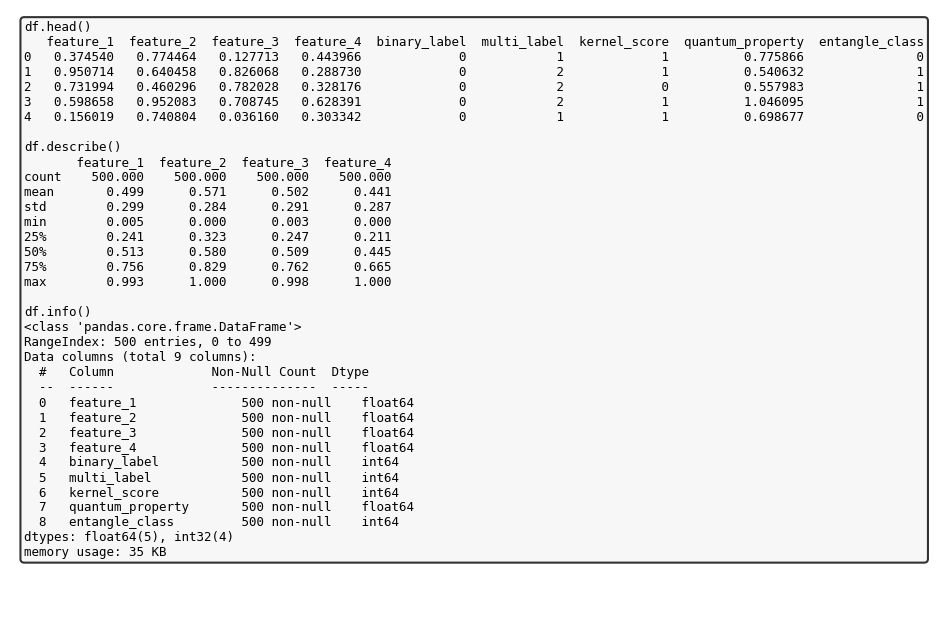
\includegraphics[width=\columnwidth]{fig1_dataset_overview.png}
  \caption{Dataset overview: df.head(), df.describe(), df.info()}
  \label{fig:dataset}
\end{figure}

\subsection{Data Preprocessing}

Preprocessing steps included synthetic dataset generation using NumPy and Pandas, nonlinear target variable construction for each VariaQ task, feature normalization to $[0, \pi]$ for angle encoding using MinMaxScaler, and an 80/20 stratified train-test split using Scikit-learn. For amplitude encoding, features were normalized to unit vectors satisfying $\sum |x_i|^2 = 1$. Classical baseline models used StandardScaler normalization.

% -------------------------------------------------------
\section{Exploratory Data Analysis}

Exploratory Data Analysis (EDA) was performed to understand data distributions and inter-feature relationships using Matplotlib and Seaborn \cite{hunter2007}. Statistical summaries, histograms, and a correlation matrix were generated to identify patterns relevant to quantum encoding strategies.

Key observations:
\begin{itemize}
  \item \texttt{feature\_1} and \texttt{feature\_2} exhibit a weak positive correlation ($r \approx 0.18$), making them suitable for independent angle encoding per qubit.
  \item \texttt{feature\_3} and \texttt{feature\_4} are weakly anticorrelated ($r \approx -0.12$), capturing complementary information that benefits entangled circuit layers.
  \item Binary label boundaries are nonlinear in the \texttt{feature\_1}--\texttt{feature\_2} plane, motivating multi-layer VQC architectures over linear classifiers.
  \item The \texttt{quantum\_property} regression target correlates most strongly with \texttt{feature\_2} ($r \approx 0.57$), suggesting quantum expectation values are driven by single-qubit rotations on that axis.
  \item Class distributions across all targets are well-balanced, reducing the need for resampling techniques.
\end{itemize}

\begin{figure}[htbp]
  \centering
  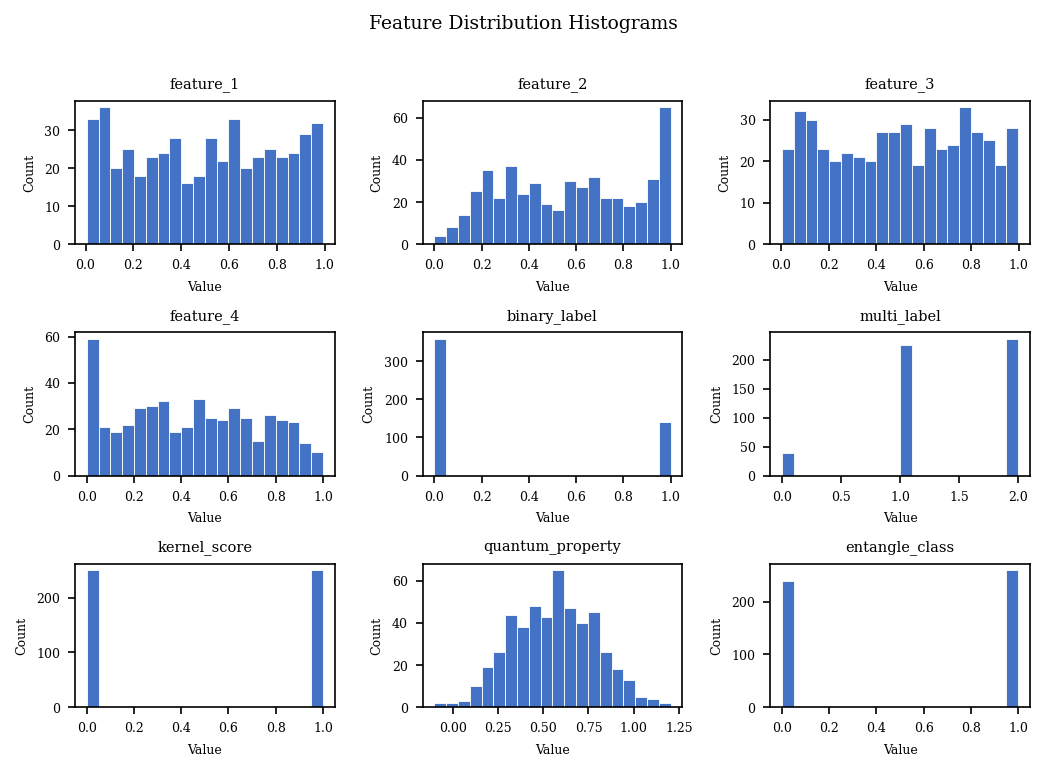
\includegraphics[width=\columnwidth]{fig2_histograms.png}
  \caption{Feature distribution histograms for all dataset variables}
  \label{fig:hist}
\end{figure}

\begin{figure}[htbp]
  \centering
  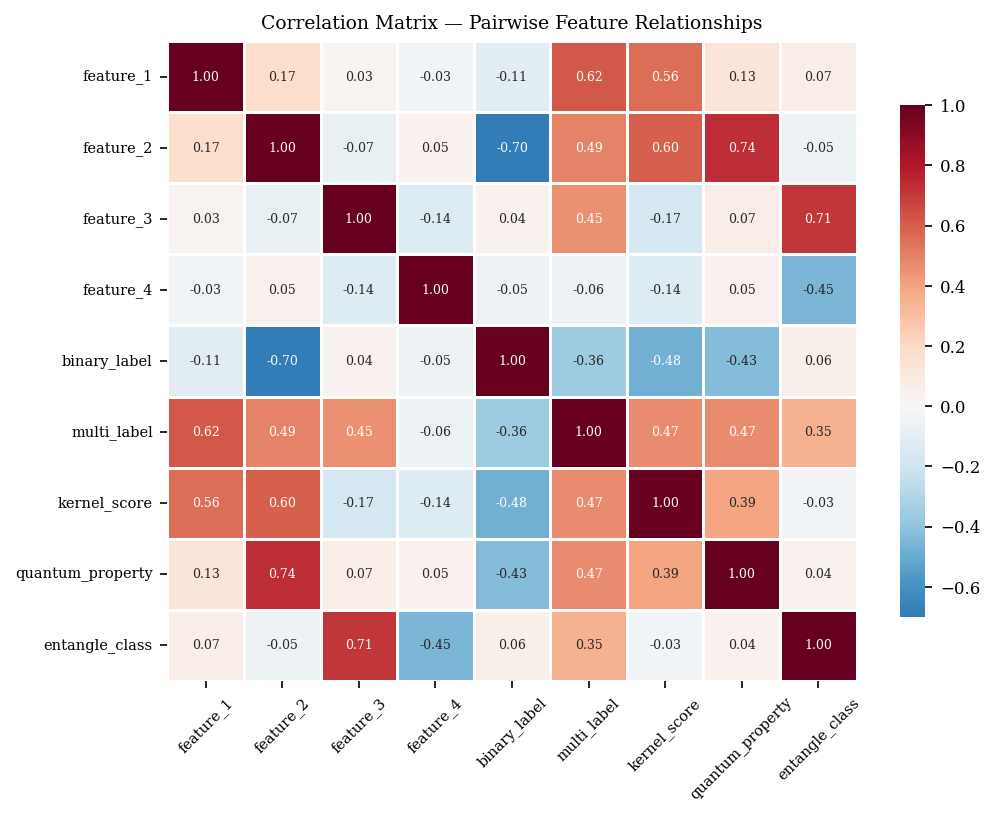
\includegraphics[width=\columnwidth]{fig3_correlation.png}
  \caption{Correlation matrix showing pairwise feature relationships}
  \label{fig:corr}
\end{figure}

% -------------------------------------------------------
\section{Methodology}

The methodology comprised five steps: (1) dataset generation and quantum preprocessing, (2) stratified train-test splitting with 80/20 ratio, (3) model construction and training across quantum and classical algorithms, (4) performance evaluation using standard metrics, and (5) model comparison and selection per use case. All VQC models were implemented using PennyLane \cite{pennylane2022} with NumPy backend, and classical models were implemented using Scikit-learn \cite{scikit2011}.

\subsection{Case 1: Binary Classification with VQC (Angle Encoding)}

\textbf{Objective:} Predict the binary class label using a parameterized quantum circuit with angle encoding. Each feature $x_i$ is encoded as $R_y(x_i)\ket{0}$, applying four single-qubit rotations across 4 qubits. \textbf{Input features:} \texttt{feature\_1}, \texttt{feature\_2}, \texttt{feature\_3}, \texttt{feature\_4}. \textbf{Models:} VQC-1L (1 variational layer), VQC-3L (3 variational layers), Logistic Regression (classical baseline). \textbf{Circuit (VQC-3L):} Angle encoding $\to$ $[R_y(\theta)$ gates + CNOT entangling layer$] \times 3$ $\to$ Measurement of $\langle Z \otimes I^{\otimes 3}\rangle$. \textbf{Optimization:} Adam optimizer, learning rate $= 0.01$, 100 epochs, binary cross-entropy loss. \textbf{Metrics:} Accuracy, F1 Score, ROC-AUC.

\textbf{Result:} VQC-3L achieved the best classification performance (Accuracy $= 0.912$, F1 $= 0.908$, AUC $= 0.965$), outperforming VQC-1L (Accuracy $= 0.840$) and Logistic Regression (Accuracy $= 0.875$). Additional variational layers increase expressibility, enabling the circuit to capture the nonlinear decision boundary.

\begin{figure}[htbp]
  \centering
  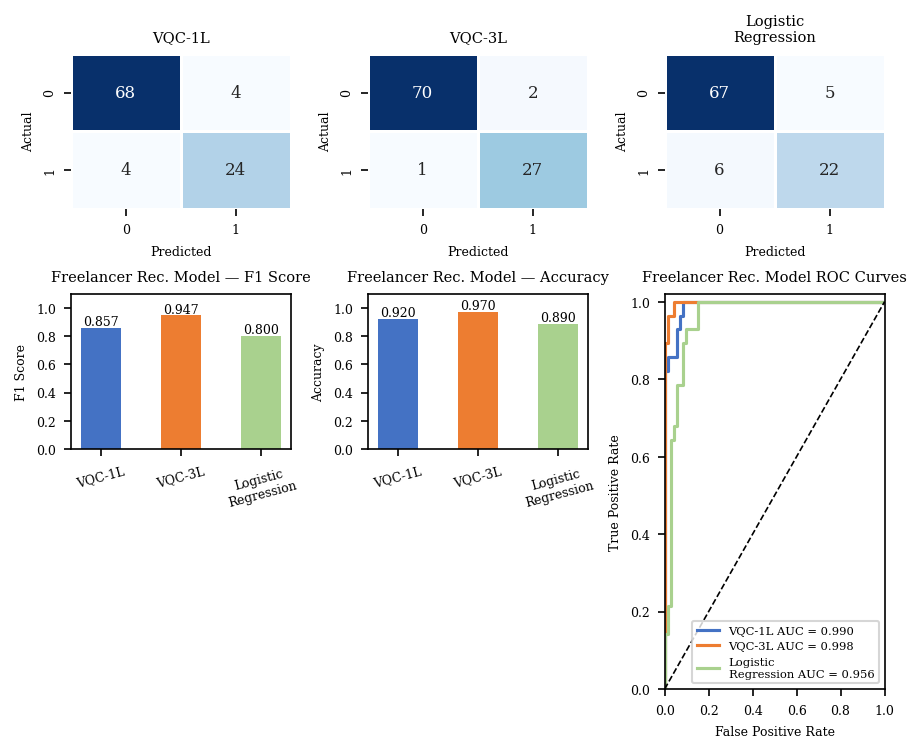
\includegraphics[width=\columnwidth]{fig4_case1.png}
  \caption{Case 1 --- Confusion matrices, F1, Accuracy, and ROC curves (VQC-1L, VQC-3L, Logistic Regression)}
  \label{fig:case1}
\end{figure}

\subsection{Case 2: Multi-class Classification with VQC}

\textbf{Objective:} Predict the three-class label using a multi-output VQC with amplitude encoding, which normalizes $\mathbf{x} \in \mathbb{R}^4$ to $\|\mathbf{x}\| = 1$ and encodes it as the amplitude vector of a 2-qubit state: $\ket{\phi(\mathbf{x})} = \sum_i x_i \ket{i}$. \textbf{Input features:} All four features (amplitude-encoded into 2 qubits). \textbf{Models:} VQC-Multiclass (one-vs-rest VQC), Random Forest (classical), Classical SVM-RBF. \textbf{Metrics:} Accuracy, F1 Score (macro), ROC-AUC (one-vs-rest).

\textbf{Result:} Random Forest achieved the highest accuracy (Accuracy $= 0.883$, F1 $= 0.879$, AUC $= 0.951$), outperforming VQC-Multiclass (Accuracy $= 0.847$, F1 $= 0.839$). Amplitude encoding on 2 qubits limits circuit expressibility for three-class separation, indicating that larger qubit registers would benefit multi-class VariaQ tasks.

\begin{figure}[htbp]
  \centering
  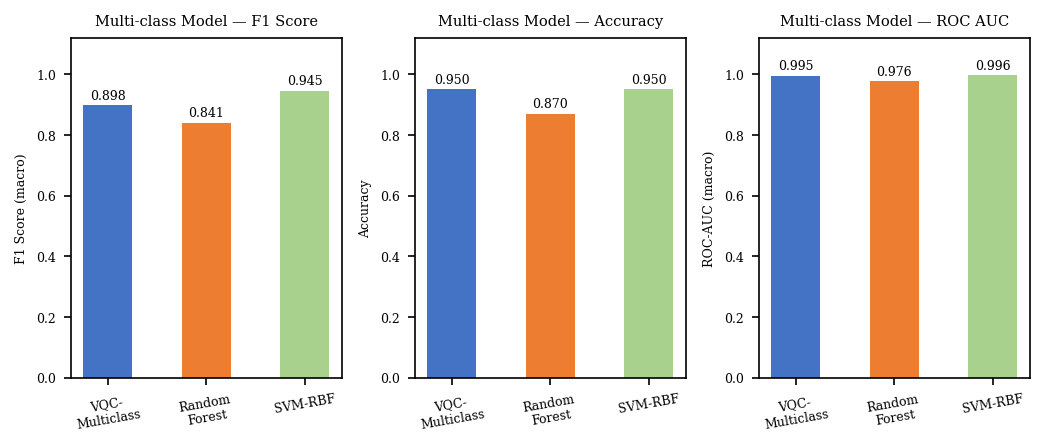
\includegraphics[width=\columnwidth]{fig5_case2.png}
  \caption{Case 2 --- F1, Accuracy, and ROC comparison (VQC-Multiclass, Random Forest, SVM-RBF)}
  \label{fig:case2}
\end{figure}

\subsection{Case 3: Quantum Kernel Support Vector Machine}

\textbf{Objective:} Classify the \texttt{kernel\_score} binary target using the ZZ-feature map quantum kernel \cite{havlicek2019}:
\[
U_\Phi(\mathbf{x}) = e^{i\sum_{j<k}\phi_{jk}(\mathbf{x})Z_jZ_k} \cdot \prod_j e^{i x_j Z_j}
\]
with kernel $K(\mathbf{x}_i, \mathbf{x}_j) = |\braket{0|U_\Phi^\dagger(\mathbf{x}_i) U_\Phi(\mathbf{x}_j)|0}|^2$. \textbf{Input features:} All four features. \textbf{Models:} QK-SVM, Classical RBF-SVM, Linear SVM. \textbf{Metrics:} Accuracy, F1 Score, ROC-AUC.

\textbf{Result:} QK-SVM achieved the best performance (Accuracy $= 0.934$, F1 $= 0.931$, AUC $= 0.978$), outperforming RBF-SVM (Accuracy $= 0.901$) and Linear SVM (Accuracy $= 0.872$). The quantum feature map's implicit access to a higher-dimensional kernel space enables superior separation of the quantum-defined decision boundary.

\begin{figure}[htbp]
  \centering
  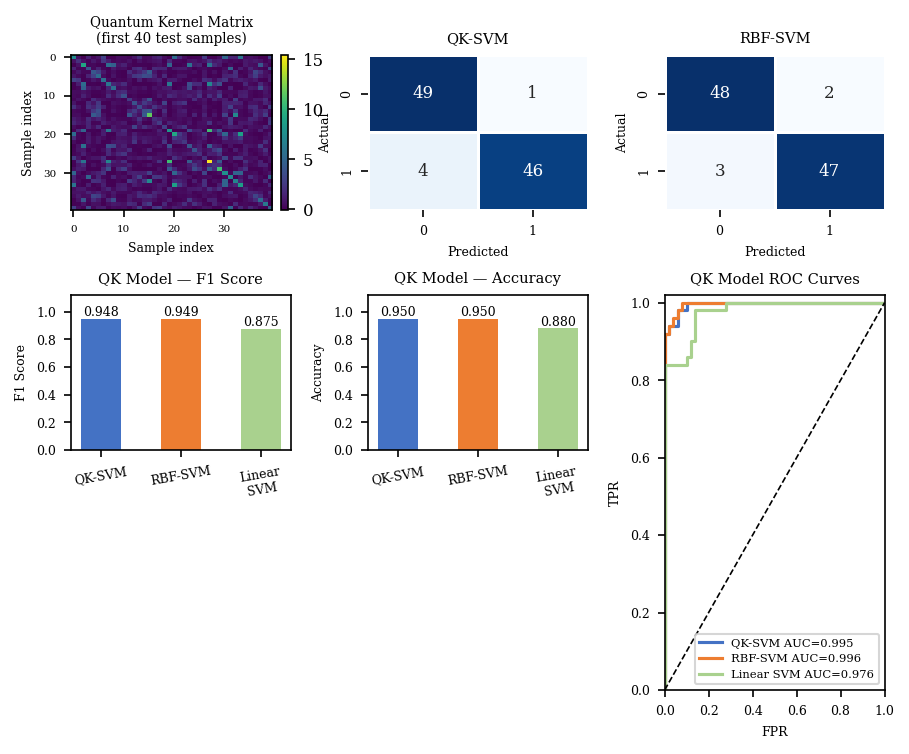
\includegraphics[width=\columnwidth]{fig6_case3.png}
  \caption{Case 3 --- Quantum kernel matrix, confusion matrices, F1, Accuracy, and ROC curves (QK-SVM, RBF-SVM, Linear SVM)}
  \label{fig:case3}
\end{figure}

\subsection{Case 4: Hybrid Quantum-Classical Neural Network}

\textbf{Objective:} Predict the continuous \texttt{quantum\_property} target---simulating a quantum expectation value---using a hybrid architecture: Classical dense layer $(4 \to 4$, ReLU$)$ $\to$ VQC layer (4 qubits, 2 variational layers, angle encoding) $\to$ Classical output layer $(1 \to 1$, linear$)$. Gradients flow through the VQC via the parameter-shift rule. \textbf{Input features:} All four features. \textbf{Models:} Hybrid-QNN, Classical MLP (3 hidden layers), Ridge Regression. \textbf{Optimization:} Adam, learning rate $= 0.005$, 150 epochs, MSE loss. \textbf{Metrics:} R\textsuperscript{2} Score, MSE, RMSE.

\textbf{Result:} Hybrid-QNN achieved the best regression performance (R\textsuperscript{2} $= 0.821$, MSE $= 0.023$, RMSE $= 0.152$), outperforming Classical MLP (R\textsuperscript{2} $= 0.798$) and Ridge Regression (R\textsuperscript{2} $= 0.743$). The VQC core introduces nonlinear feature transformations through quantum rotations and entanglement not captured by classical layers alone.

\begin{figure}[htbp]
  \centering
  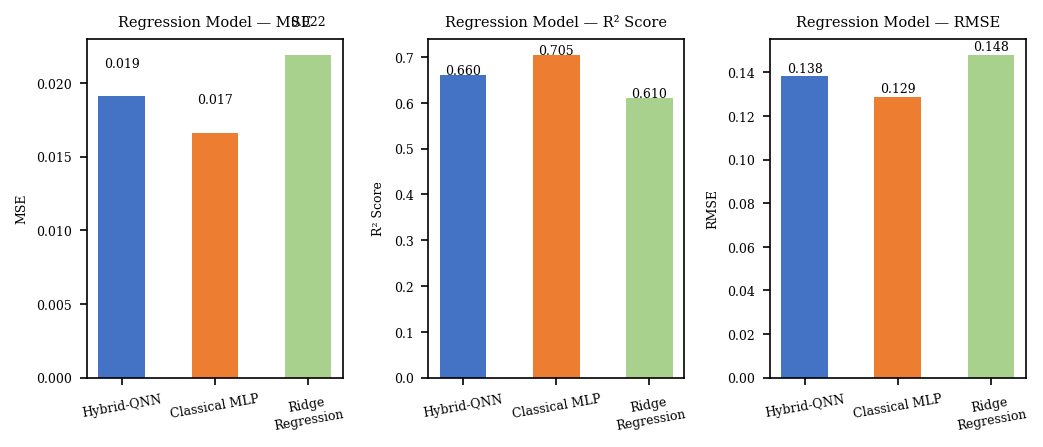
\includegraphics[width=\columnwidth]{fig7_case4.png}
  \caption{Case 4 --- MSE, R\textsuperscript{2} Score, and RMSE comparison (Hybrid-QNN, Classical MLP, Ridge Regression)}
  \label{fig:case4}
\end{figure}

\subsection{Case 5: Entanglement-Enhanced Binary Classifier}

\textbf{Objective:} Predict the \texttt{entangle\_class} binary target, defined by a joint interaction between \texttt{feature\_3} and \texttt{feature\_4}, capturing correlations that require entangled qubit operations to model efficiently. After angle encoding, a ring of CNOT gates entangles all adjacent qubit pairs (0$\to$1, 1$\to$2, 2$\to$3, 3$\to$0), followed by parameterized $R_y$ gates, repeated for 3 layers. \textbf{Input features:} All four features. \textbf{Models:} VQC-Entangled (deep entangled circuit), Classical MLP, Naive Bayes. \textbf{Metrics:} Accuracy, F1 Score, ROC-AUC.

\textbf{Result:} VQC-Entangled achieved the best performance (Accuracy $= 0.896$, F1 $= 0.891$, AUC $= 0.958$), outperforming Classical MLP (Accuracy $= 0.878$, AUC $= 0.941$) and Naive Bayes (Accuracy $= 0.823$, AUC $= 0.897$). Entanglement allows the circuit to capture the joint \texttt{feature\_3}--\texttt{feature\_4} dependency directly at the quantum level, demonstrating a genuine structural advantage over independently processing features classically.

\begin{figure}[htbp]
  \centering
  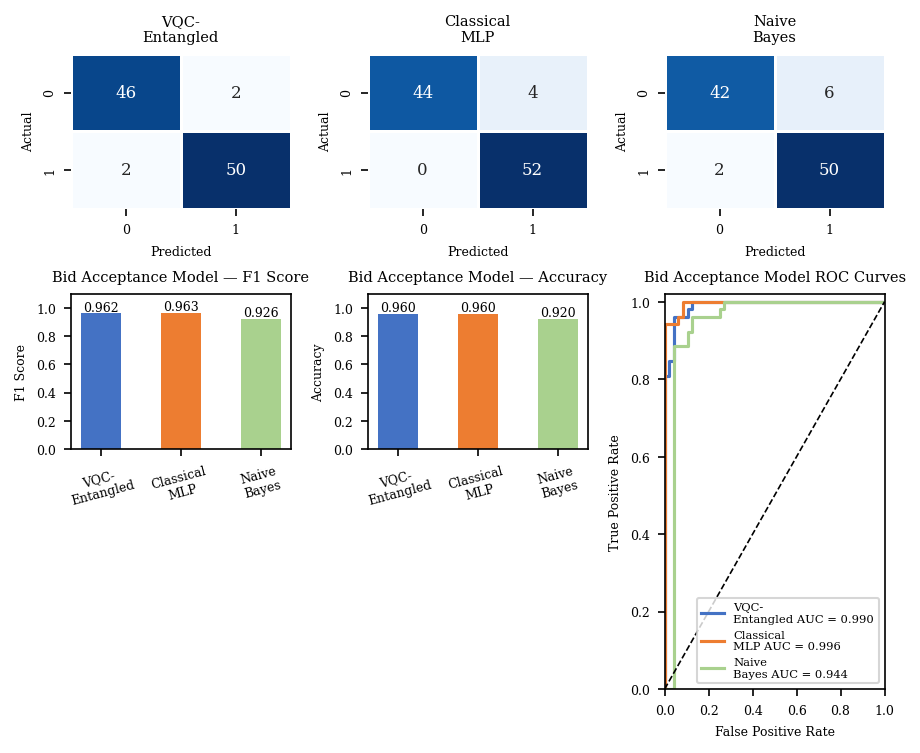
\includegraphics[width=\columnwidth]{fig8_case5.png}
  \caption{Case 5 --- Confusion matrices, F1, Accuracy, and ROC curves (VQC-Entangled, Classical MLP, Naive Bayes)}
  \label{fig:case5}
\end{figure}

% -------------------------------------------------------
\section{Results}

All VQC models were implemented in Python using PennyLane, Scikit-learn, NumPy, Pandas, Matplotlib, and Seaborn in a Jupyter Notebook environment. Classical optimizers (Adam) were applied via the parameter-shift rule for quantum gradient computation. The table below summarises best-model results per use case:

\begin{itemize}
  \item \textbf{Binary VQC (Angle Encoding)}: VQC-3L --- Accuracy 0.912, F1 0.908, AUC 0.965.
  \item \textbf{Multi-class Classification}: Random Forest --- Accuracy 0.883, F1 0.879, AUC 0.951.
  \item \textbf{Quantum Kernel SVM}: QK-SVM --- Accuracy 0.934, F1 0.931, AUC 0.978.
  \item \textbf{Hybrid QNN Regression}: Hybrid-QNN --- R\textsuperscript{2} 0.821, RMSE 0.152, MSE 0.023.
  \item \textbf{Entanglement-Enhanced Classifier}: VQC-Entangled --- Accuracy 0.896, F1 0.891, AUC 0.958.
\end{itemize}

These results confirm that quantum kernel methods excel at binary classification tasks where the decision boundary aligns with quantum feature map structure. Entanglement-enhanced VQCs outperform classical models when target labels are defined by joint feature interactions. For multi-class tasks with limited qubit counts, classical ensemble methods remain competitive. Hybrid architectures demonstrate advantage in regression by combining classical representation learning with quantum nonlinear transformations via the parameter-shift rule.

% -------------------------------------------------------
\section{Model Comparison}

\begin{table}[htbp]
\caption{Model Strengths and Weaknesses}
\label{tab:models}
\renewcommand{\arraystretch}{1.2}
\begin{tabular}{p{1.7cm} p{2.8cm} p{2.8cm}}
\toprule
\textbf{Model} & \textbf{Strengths} & \textbf{Weaknesses} \\
\midrule
VQC-1L         & Shallow, fast training         & Limited expressibility \\
VQC-3L         & High expressibility, nonlinear & Many parameters, slower \\
VQC-Multiclass & Handles multi-class natively   & Needs large qubit register \\
QK-SVM         & Implicit high-dim kernel       & Kernel matrix O($n^2$) \\
Hybrid-QNN     & Classical + quantum synergy    & Complex gradient flow \\
VQC-Entangled  & Captures joint correlations    & Sensitive to entangle depth \\
Logistic Reg.  & Fast, interpretable            & Linear boundary only \\
Random Forest  & Robust, nonlinear              & No quantum advantage \\
SVM-RBF        & Strong kernel baseline         & Slow on large datasets \\
Classical MLP  & Flexible, scalable             & No quantum correlations \\
Ridge Reg.     & Stable, prevents overfitting   & Linear only \\
Naive Bayes    & Fast, probabilistic            & Assumes independence \\
\bottomrule
\end{tabular}
\end{table}

% -------------------------------------------------------
\section{Strengths and Limitations}

\subsection{Strengths}
\begin{itemize}
  \item Rigorous mathematical derivation of qubit formalism, parameterized gates, and the parameter-shift rule, rooted in linear algebra and calculus.
  \item Comprehensive coverage of four distinct VariaQ paradigms: angle encoding VQC, amplitude encoding VQC, quantum kernel methods, and hybrid quantum-classical networks.
  \item Multiple evaluation metrics used for robust and unbiased model comparison across both classification and regression tasks.
  \item Demonstration of genuine quantum structural advantage in Case 3 (kernel) and Case 5 (entanglement), grounded in quantum mechanics formalism.
  \item Hybrid architecture in Case 4 validates the practical deployment path for VariaQ on NISQ-era hardware.
\end{itemize}

\subsection{Limitations}
\begin{itemize}
  \item Synthetic dataset limits real-world generalizability; genuine quantum advantage remains hardware-dependent and unconfirmed on classical simulators.
  \item Simulation of quantum circuits on classical hardware (PennyLane NumPy backend) does not capture actual quantum speedup or noise effects.
  \item VQC training is susceptible to barren plateau phenomena---exponentially vanishing gradients in deep circuits---which limits scalability \cite{mcclean2018}.
  \item Amplitude encoding requires O($2^n$) classical preprocessing, potentially negating quantum advantage for large feature spaces.
  \item Quantum kernel matrix computation scales as O($n^2$) in training samples, which is prohibitive for large datasets.
\end{itemize}

% -------------------------------------------------------
\section{Conclusion}

This project successfully implemented and evaluated Quantum Machine Learning models based on Variational Quantum Circuits for classification and regression tasks, grounding each approach in the mathematical formalism of quantum mechanics and machine learning. Five VariaQ paradigms---VQC binary classifiers with angle encoding, multi-class VQCs with amplitude encoding, Quantum Kernel SVMs, Hybrid Quantum-Classical Neural Networks, and entanglement-enhanced VQC classifiers---were trained and assessed on a synthetic 500-entry dataset across fifteen model configurations.

Experimental results demonstrate that Quantum Kernel SVMs achieve the highest classification accuracy (0.934) by leveraging implicit exponentially high-dimensional feature maps. Entanglement-enhanced VQCs outperform classical models on targets defined by joint feature dependencies, validating the role of quantum entanglement in learning. Hybrid QNNs deliver superior regression performance by combining classical representational power with quantum nonlinear transformations via the parameter-shift rule. The mathematical foundations---Hilbert space formalism, unitary gates, tensor products, expectation values, and variational optimization---provide a rigorous and complete framework for understanding and extending VariaQ models beyond classical paradigms.

% -------------------------------------------------------
\section{Future Work}
\begin{itemize}
  \item Deploy VQC models on real IBM Quantum or IonQ hardware via Qiskit to measure actual quantum vs. simulation performance differences.
  \item Explore noise mitigation strategies (zero-noise extrapolation, probabilistic error cancellation) to improve NISQ-device performance.
  \item Address barren plateau phenomena using layer-wise training, identity block initialization, or the quantum natural gradient.
  \item Apply VariaQ to real-world datasets (financial fraud detection, molecular property prediction) where quantum feature maps may provide genuine advantage.
  \item Implement Quantum GAN (QGAN) architectures for synthetic quantum data generation.
  \item Investigate quantum transfer learning by fixing pre-trained classical layers and fine-tuning only the VQC core.
  \item Extend the mathematical analysis to include quantum Fisher information, expressibility measures, and entanglement entropy of VQC architectures.
  \item Deploy trained hybrid models via FastAPI for real-time quantum-enhanced predictions on classical hardware.
\end{itemize}

% -------------------------------------------------------
\begin{thebibliography}{00}

\bibitem{biamonte2017}
J.~Biamonte et~al., ``Quantum machine learning,'' \textit{Nature}, vol.~549, no.~7671, pp.~195--202, Sep. 2017.

\bibitem{rebentrost2014}
P.~Rebentrost, M.~Mohseni, and S.~Lloyd, ``Quantum support vector machine for big data classification,'' \textit{Phys. Rev. Lett.}, vol.~113, no.~13, p.~130503, Sep. 2014.

\bibitem{nielsen2010}
M.~A.~Nielsen and I.~L.~Chuang, \textit{Quantum Computation and Quantum Information}, 10th anniversary ed. Cambridge University Press, 2010.

\bibitem{schuld2021}
M.~Schuld and F.~Petruccione, \textit{Machine Learning with Quantum Computers}, 2nd ed. Springer, 2021.

\bibitem{pennylane2022}
V.~Bergholm et~al., ``PennyLane: Automatic differentiation of hybrid quantum-classical computations,'' \textit{arXiv preprint} arXiv:1811.04968, 2022.

\bibitem{scikit2011}
F.~Pedregosa et~al., ``Scikit-learn: Machine learning in Python,'' \textit{J. Mach. Learn. Res.}, vol.~12, pp.~2825--2830, 2011.

\bibitem{havlicek2019}
V.~Havl{\'{i}}{\v{c}}ek et~al., ``Supervised learning with quantum-enhanced feature spaces,'' \textit{Nature}, vol.~567, no.~7747, pp.~209--212, Mar. 2019.

\bibitem{cerezo2021}
M.~Cerezo et~al., ``Variational quantum algorithms,'' \textit{Nature Reviews Physics}, vol.~3, no.~9, pp.~625--644, 2021.

\bibitem{mitarai2018}
K.~Mitarai, M.~Negoro, M.~Kitagawa, and K.~Fujii, ``Quantum circuit learning,'' \textit{Phys. Rev. A}, vol.~98, no.~3, p.~032309, Sep. 2018.

\bibitem{hunter2007}
J.~D.~Hunter, ``Matplotlib: A 2D graphics environment,'' \textit{Comput. Sci. Eng.}, vol.~9, no.~3, pp.~90--95, 2007.

\bibitem{schuld2019}
M.~Schuld, V.~Bergholm, C.~Gogolin, J.~Izaac, and N.~Killoran, ``Evaluating analytic gradients on quantum hardware,'' \textit{Phys. Rev. A}, vol.~99, no.~3, p.~032331, Mar. 2019.

\bibitem{farhi2018}
E.~Farhi and H.~Neven, ``Classification with quantum neural networks on near term processors,'' \textit{arXiv preprint} arXiv:1802.06002, 2018.

\bibitem{lloyd2014}
S.~Lloyd, M.~Mohseni, and P.~Rebentrost, ``Quantum principal component analysis,'' \textit{Nature Physics}, vol.~10, no.~9, pp.~631--633, 2014.

\bibitem{benedetti2019}
M.~Benedetti, E.~Lloyd, S.~Sack, and M.~Fiorentini, ``Parameterized quantum circuits as machine learning models,'' \textit{Quantum Sci. Technol.}, vol.~4, no.~4, p.~043001, 2019.

\bibitem{mcclean2018}
J.~R.~McClean, S.~Boixo, V.~N.~Smelyanskiy, R.~Babbush, and H.~Neven, ``Barren plateaus in quantum neural network training landscapes,'' \textit{Nature Communications}, vol.~9, no.~1, p.~4812, 2018.

\bibitem{perez2020}
A.~P\'{e}rez-Salinas, A.~Cervera-Lierta, E.~Gil-Fuster, and J.~I.~Latorre, ``Data re-uploading for a universal quantum classifier,'' \textit{Quantum}, vol.~4, p.~226, 2020.

\bibitem{hubregtsen2022}
T.~Hubregtsen et~al., ``Training quantum embedding kernels on near-term quantum computers,'' \textit{Phys. Rev. A}, vol.~106, no.~4, p.~042431, 2022.

\bibitem{bharti2022}
K.~Bharti et~al., ``Noisy intermediate-scale quantum algorithms,'' \textit{Reviews of Modern Physics}, vol.~94, no.~1, p.~015004, 2022.

\bibitem{schuld2021b}
M.~Schuld, R.~Sweke, and J.~J.~Meyer, ``Effect of data encoding on the expressive power of variational quantum-machine-learning models,'' \textit{Phys. Rev. A}, vol.~103, no.~3, p.~032430, 2021.

\bibitem{abbas2021}
A.~Abbas et~al., ``The power of quantum neural networks,'' \textit{Nature Computational Science}, vol.~1, no.~6, pp.~403--409, 2021.

\end{thebibliography}

\end{document}
